\documentclass{amsart}
\usepackage[utf8]{inputenc}

\usepackage{amsmath,amssymb,amsthm}
\usepackage{comment}
\usepackage{hyperref}
\usepackage{pgf,tikz}
%\usepackage{showkeys}

\usetikzlibrary{arrows}
\usetikzlibrary{arrows.meta}

\newcommand{\RR}{\mathbb R}
\newcommand{\CC}{\mathbb C}
\newcommand{\NN}{\mathbb N}
\newcommand{\ZZ}{\mathbb Z}

\renewcommand{\H}{\mathcal H}
\newcommand{\eps}{\varepsilon}

\newcommand{\loc}{\mathrm{loc}}

\renewcommand{\vec}[1]{\mathbf{#1}}
\newcommand{\abs}[1]{\left\vert #1 \right\vert}
\newcommand{\Abs}[1]{\left\Vert #1 \right\Vert}
\newcommand{\enclose}[1]{\left(#1\right)}
\newcommand{\Enclose}[1]{\left[#1\right]}
\newcommand{\ENCLOSE}[1]{\left\{#1\right\}}
\newcommand{\weakstarto}{{\stackrel{*}{\rightharpoonup}}}

\newcommand{\St}{\mathrm{St}}
\newcommand{\M}{\mathcal{M}}
\renewcommand{\H}{\mathcal{H}}
\newcommand{\dist}{\mathrm{dist}}
\newcommand{\co}{\mathrm{co}}
\renewcommand{\S}{\mathcal{S}}

\newtheorem{theorem}{Theorem}[section]
\newtheorem{proposition}[theorem]{Proposition}
\newtheorem{conjecture}[theorem]{Conjecture}
\newtheorem{lemma}[theorem]{Lemma}
\newtheorem{corollary}[theorem]{Corollary}
\newtheorem{assumption}[theorem]{Assumption}
\newtheorem{problem}[theorem]{Problem}
\newtheorem{openpb}[theorem]{Open Problem}
\theoremstyle{definition}
\newtheorem{definition}[theorem]{Definition}
\theoremstyle{remark}
\newtheorem{remark}[theorem]{Remark}
\newtheorem{example}[theorem]{Example}

\author[Paolini]{Emanuele Paolini} 
\address[Emanuele Paolini]{Dipartimento di Matematica, Universit\`a di Pisa \\
	Largo Bruno Pontecorvo 5 \\ I-56127, Pisa}
\email[Emanuele Paolini]{emanuele.paolini@unipi.it}

\author[Stepanov]{Eugene Stepanov}
\address[Eugene Stepanov]{%
  Scuola Normale Superiore, Piazza dei Cavalieri 6, Pisa, Italy
  \and 
  St.Petersburg Branch of the Steklov Mathematical Institute of the Russian Academy of Sciences,
	St.Petersburg, Russia
	%\and
	%Department of Mathematical Physics, Faculty of Mathematics and Mechanics,
	%St. Petersburg State University, Universitetskij pr.~28, Old Peterhof,
	%198504 St.Petersburg, Russia%, email: stepanov.eugene@gmail.com
	%\and ITMO University
	\and
	Faculty of Mathematics, Higher School of Economics, Moscow
}
\email[Eugene Stepanov]{stepanov.eugene@gmail.com}

\thanks{
	%Data sharing not applicable to this article as no datasets were generated or analysed during the current study.
	The first author is member of the INDAM/GNAMPA 
  and is supported by the PRIN Project 2019/24.
%	The work of the third author has been partially financed by the 
%  RFBR grant \#20-01-00630 A
}
\subjclass[2010]{Primary 49Q20, 49Q05, 49Q10. Secondary 05C63.}
\keywords{Steiner problem, Steiner tree, fractal set}
\date{\today}

\title{On the Steiner tree connecting a fractal set}

\begin{document}

\begin{abstract}
We construct an example of an infinite planar embedded self-similar binary tree  
$\Sigma$ which is the essentially unique solution to the Steiner problem of finding 
the shortest connection of a given planar self-similar fractal set $C$
of positive Hausdorff dimension.
The set $C$ can be considered the set of \emph{leaves}, or the ``boundary``,
of the tree $\Sigma$,
so that $\Sigma$ is an \emph{irreducible} solution to the Steiner problem
with datum $C$ (i.e.\ $\Sigma\setminus C$ is connected).
\end{abstract}

\maketitle

\section{Introduction}

Let $C$ be a subset of $\RR^2$.
The Steiner problem with datum $C$ consists of finding a set $S\subset \RR^2$ 
such that $S\cup C$ is connected and $\H^1(S)$ is minimal where $\H^1$ stands 
for the $1$-dimensional Hausdorff measure (i.e.\ the length of the set).
Usually this problem is considered for the case when $C$ is the finite 
set and in this setting it becomes a problem of combinatorial geometry. 
The Steiner problem goes back to Jarník and Kössler \cite{JarKos34} 
(although some of its particular cases are much more ancient, for instance 
when $C$ is the set of the three vertices of a triangle the problem was 
stated already by Fermat and solved by Torricelli).
The problem is computationally hard and relatively few explicit solutions 
are known, especially in the cases when the number of points is large.

However the problem is important for the more general setting of possibly infinite 
sets $C$. 
Moreover finding explicit solutions for an infinite $C$ may shed light on 
the solutions to finite sets with an arbitrarily large number of points.
One natural question that has arosen in this context is 
whether there exists a planar irreducible Steiner tree $S$ connecting an uncountable 
and possibly fractal set of points $C$ 
(we say that $S$ is irreducible if $S\setminus C$ is 
connected).
A very similar question,
that of existence of irreducible Steiner sets with the topology 
of a binary tree for a finite set of points $C$ with arbitrarily 
large number of points, has been answered positively by Ivanov and 
Tuzhilin \cite{IvaTuz94} by means of an abstract construction.
Further an explicit construction of such a tree has been constructed 
in \cite{PaoSteTep15}.
Namely, the set $C$ consists of a \emph{root} $H$ and uncountably many
points (\emph{leaves}) which together give a totally disconnected perfect set 
(i.e.\ every connected component is a point, but the points are not isolated).
No segment of $S$
touches the leaves, while every leaf is an accumulation point of
segments of $S$.
The infinite tree $S$ 
is composed by a \emph{trunk} of
some length $\ell$ which splits at angles of 120 degrees 
into two branches of length $\lambda_1 \ell$ 
both of which split further at the same angles into two branches of length
$\lambda_1\lambda_2\ell$ and so on (see Figure~\ref{fig:tree}).
\begin{figure}
  \centering 
  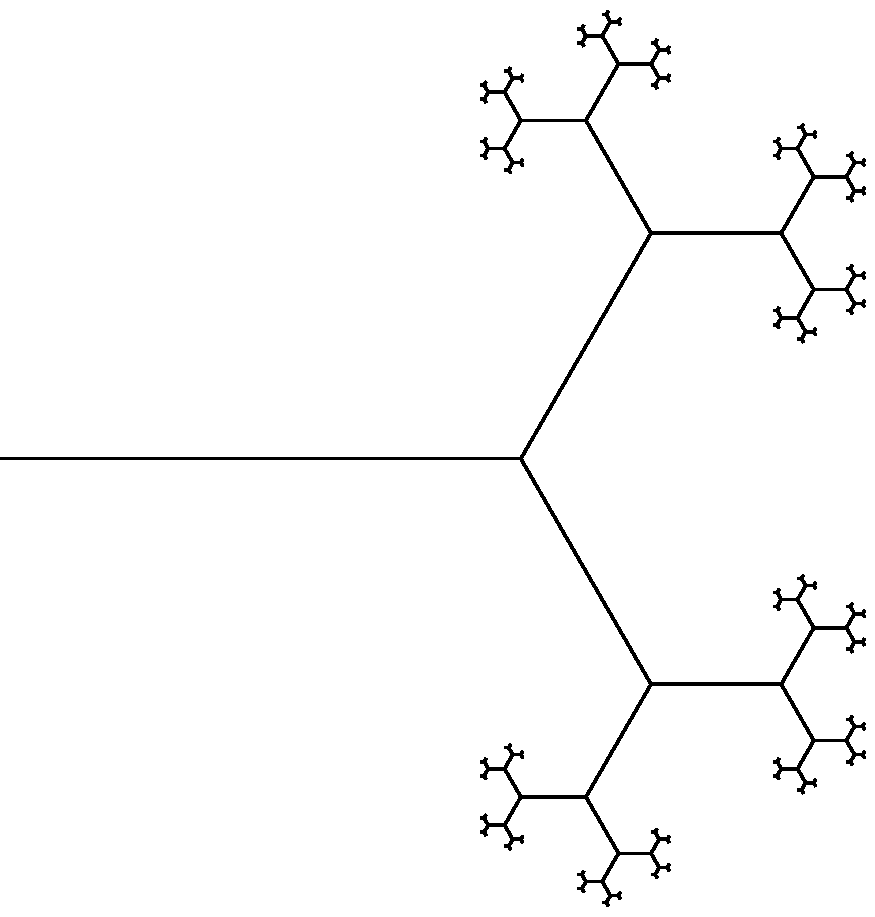
\includegraphics[height=6cm]{tree.pdf}
  \label{fig:tree}
  \caption{The self-similar tree $S$ with a countable 
  number of triple junctions and an uncountable number 
  of leaves which are the limit points of the triple 
  junctions.}
\end{figure}
% Our proof requires that the sequence $\{\lambda_j\}$ vanish rather quickly (in fact, al least be summable).
% It is an open question if in the case of a
% constant sequence $\lambda_j=\lambda$ (with $\lambda>0$ small enough) the same construction
% still provides a Steiner tree. This seems to be quite interesting
% since the resulting tree would be, in that case, a \emph{self-similar}
% fractal.

In \cite{PaoSteTep15} it has been proven that 
the suggested tree is in fact the solution (and even the unique one) 
to the Steiner problem when the sequence of coefficients $\lambda_k$
is small and rapidly decreasing to zero (in particular summable).
In such a situation the set $C$ though being uncountable 
has zero Hausdorff dimension.
The natural original question, whether this construction is also valid 
for fractal self-similar $C$ (i.e.\ when the coefficients are constant,
i.e.\ $\lambda_j=\lambda$ for all $j$)
was left open.
In the attempt to solve it, a 
completely new and different method, based on special group valued calibrations,
to check whether the given set $S$ is a solution to the Steiner problem,
has been developed in~\cite{MarMas16a}.
In \cite{MarMas16b} the authors also show an example 
of an infinite \emph{irrigation} tree which is a solution to
a ramified transportation problem similar to the Steiner problem.
The method itself is very useful and can be applied in many situations.
However it failed in this particular problem.
A breakthrough has been provided by the recent preprint \cite{CheTep23}
where the authors provide a much simpler symmetry based argument to show that for 
sufficiently small but constant coefficients the above construction 
gives in fact an irreducible Steiner tree for a set $C$ 
of positive Hausdorff dimension.
However this construction unfortunately does not provide uniqueness of 
the minimizer leaving open the possibility of having other solutions 
different from the conjectured one.
In this paper 
we close the original question of both existence and uniqueness.
To do so we develop a method which in particular uses 
also a further simplification and a generalization of 
the idea developed in \cite{CheTep23}.
Moreover since we do not use the symmetry argument anymore our method 
could be applied even to non symmetric trees.

To be more precise, 
let $\RR^2$ be identified with the complex plane $\CC$
and given $\lambda>0$, 
consider $f_j(z) = 1 + \theta_j z$,
where $\theta = \lambda e^{(-1)^j i \frac \pi 3}$,
for $j=1,2$. 
The affine map $f_j$ is the composition of a rotation,
rescaling and translation. 
Let $A$ be the only non-empty compact set such that 
\[
  A = f_1(A) \cup f_2(A).  
\]
One can check that $A$ is the limit, 
in the sense of Hausdorff distance,
of the finite sets $A_N$ where $A_N:=\ENCLOSE{f_{j_1}(f_{j_2}(\dots f_{j_N}(0)))\colon 
j_1,j_2, \dots, j_N \in \ENCLOSE{1,2}}$.
We are going to prove that if $\lambda$ is sufficiently 
small then 
for $C:=\ENCLOSE{H}\cup A$, with $H=0$, the closure $\bar S$ of any solution 
$S$ to the Steiner problem 
is connected and is equal to the binary self-similar 
tree $\Sigma$ defined by the recurrence equation
\[
  \Sigma = [0,1] \cup f_1(\Sigma) \cup f_2(\Sigma).
\]
Equivalently one can define $\Sigma$ as
\[
  \Sigma := \overline{\bigcup_{N \in \NN}  
  \bigcup\ENCLOSE{f_{j_1}\circ \dots \circ f_{j_N}([0,1])\colon 
  j_1, \dots, j_N \in \ENCLOSE{1,2}}}.
\]

\section{Notation and preliminaries}

Let $\St(C)$ be the family of all sets $S$ such that 
$S\cup C$ is connected and 
let $\M(C)$ be the subset of $\St(C)$ of sets $S$ 
with minimal (possibly infinite) length $\H^1(S)$.

For a set $S\subset \RR^2$ we denote by $\bar S$ 
its closure and by $\partial S$ its topological boundary.
If $x\in \RR^2$ and $\rho>0$ then we let $B_\rho(x)\subset \RR^2$ 
be the open ball of radius 
$\rho$ centered at $x$.
When $x\in \RR^2$, $S,S_1,S_2$ subsets of $\RR^2$
we also write
\begin{align*}
  \dist(x,S)
    &:=\inf\ENCLOSE{\abs{x-y}:y\in S},\\
  \dist(S_1,S_2) 
    &:= \inf\ENCLOSE{\abs{x-y}\colon x\in S_1, y\in S_2}.
\end{align*}
For $P,Q\in \RR^2$ we denote by $[PQ]$ the closed straight line 
segment with endpoints $P$ and $Q$ and by $\abs{PQ}$ its length.

% \subsection{Construction}
% 
% \begin{conjecture}
%   The result is valid for any $\lambda$ smaller than 
%   the solution to the following equation:
%   \[
%     1+\frac\lambda 2 
%     - \frac {\lambda^2} 2 \frac{1+2\lambda}{1-\lambda^2}
%     +\sqrt 3 \lambda \frac{1 - \frac{\lambda^2}{1-\lambda}}{1-2\lambda}
%     = \frac{1}{1-2\lambda}.
%   \]
%   Which is (maybe) equivalent to
%   \[
%   (6-2\sqrt 3)\lambda^3 + (3-4\sqrt 3)\lambda^2 - 3\lambda + 2\sqrt 3 - 1 =0  
%   \]
%   which has solution $\lambda\approx 0.43276$.
% 
% \end{conjecture}

\subsection{Auxiliary lemmata}

In the following proposition we state some known facts about 
solutions to the Steiner problem collected from \cite{PaoSte12}
and \cite{IvaTuz94}.

\begin{proposition}[known facts about minimizers]\label{prop:PaoSte}
  Let $C\subset \RR^n$ be a compact set.
  Then $\M(C)\neq \emptyset$. If $S\in \M(C)$
  with $\H^1(S)<+\infty$
  then the following assertions hold.
  \begin{itemize}
    \item[(i)] $S\cup C$ is compact, 
    hence $\bar S \setminus S \subset C$;
    \item[(ii)] the closure of every connected component of $S$     
    is a topological tree 
    (contains no subset homeomorphic to $\mathbb S^1$)
    with endpoints\footnote{%
    When $S$ is a compact topological tree, then $x\in S$ is an endpoint 
    of $S$ if and only if $S\setminus \ENCLOSE{x}$ is connected.} 
    on $C$ and with at most one endpoint 
    on each connected component of $C$;
    \item[(iii)] for all $x\in S\setminus C$ and all 
    $\rho < \dist(x,C)$ the set $S\cap \bar B_\rho(x)$ 
    is the union of a finite number of straight line 
    segments which meet in triple points with equal 
    angles of 120 degrees and have endpoints in 
    $\partial B_\rho(x)$.
  \end{itemize}
\end{proposition}

The following lemma is also taken from~\cite[lemma~2.6]{PaoSte12}.

\begin{lemma}\label{lm:connected}
If $S$ is connected and $\H^1(S)<+\infty$ then $\H^1(S) = \H^1(\bar S)$.
\end{lemma}

We also need the following lemmata for the case when the set to 
be connected is not compact but contains a line.

\begin{lemma}\label{lm:exists}
  Let $C$ be a compact subset of $\RR^2$ and $\ell$ be a straight line.
  Then $\M(\ell\cup C)\neq \emptyset$.
  If $C$ is also totally disconnected, $C\cap \ell=\emptyset$ 
  and $S\in \M(\ell\cup C)$  
  then $\bar S \supset C$.
  If moreover $\H^1(S)<+\infty$ and $\H^1(C)=0$ 
  then $\bar S\in \M(\ell\cup C)$.
\end{lemma}
\begin{proof}
  Take a compact connected segment $\sigma\subset \ell$ such that 
  the orthogonal projection of $C$ on $\ell$ is contained 
  in $\sigma$. 
  Then $\sigma\cup C$ is compact and by 
  \cite{PaoSte12} we know that 
  $\M(\sigma \cup C)\neq \emptyset$.
  For all $\Sigma \in \St(\ell\cup C)$ we have that its projection 
  $\tilde \Sigma$ 
  onto the convex hull of $\sigma\cup C$ is in $\St(\sigma\cup C)$
  and $\H^1(\tilde \Sigma)\le \H^1(\Sigma)$.
  Hence $\M(\ell\cup C)\supset \M(\sigma\cup C)\neq \emptyset$ as claimed.

  To prove the second part note that if $C$ is totally disconnected 
  then for every $x\in C$ one has $x\in \bar S$ otherwise 
  $S\cup C\cup \ell$ cannot be connected. 
  Therefore $C\subset \bar S$. 
  
  For the last claim notice that $\bar S\cap \ell$ is a finite set.
  In fact the number of connected components of $S$ arriving at $\ell$ 
  is finite since every such component must touch also points of $C$ 
  and hence has length at least $\dist(C,\ell)$.  
  Hence these components cannot be infinitely many,
  since otherwise we would have $\H^1(S)=+\infty$.
  In view of Proposition~\ref{prop:PaoSte}(ii) 
  the closure of every connected component 
  of $S\in\M(C\cup \sigma)$ 
  has at most one point on $\sigma$, showing that the set 
  $W:=\bar S\cap \sigma = \bar S \cap \ell$ 
  is finite.

  Moreover $\bar S \setminus S \subset C\cup W$ because 
  $S\cup C\cup \sigma$ is compact by Proposition~\ref{prop:PaoSte}(i).
  When $\H^1(C)=0$ this implies $\H^1(\bar S)=\H^1(S)$ and hence 
  $\bar S\in \M(\ell\cup C)$.
\end{proof}

\begin{lemma}\label{lm:base}
  Let $\ell$ be a line, $\rho>0$, 
  $r=2\rho/\sqrt 3$.
  Let $P$ be a point such that $\dist(P,\ell)>3r$
  and let $C$ be a compact subset of $\bar B_\rho(P)$.
  Let $S \in \M(\ell\cup C)$ 
  (such $S$ exists in view of Lemma~\ref{lm:exists})
  and suppose $\H^1(S)<+\infty$.
  Then there exists a point $Q\in \partial B_r(P)$ 
  and a point $H\in \ell$
  such that $\bar S\setminus B_r(P) = [HQ]$.
  Moreover $[HQ]$ is perpendicular to $\ell$.
\end{lemma}
\begin{proof}
  We claim that $S\setminus B_r(P)$ belongs to 
  a single connected component of $S$. 
  In fact, if not, there are two different connected components 
  $S_1$ and $S_2$ of $S$ which have some points outside of 
  $B_r(P)$. 
  Their closures must have points in $\ell$ otherwise 
  they would be contained in the convex hull of $C\subset B_r(P)$.
  By Proposition~\ref{prop:PaoSte}(ii) we know  
  that $\bar S_1$ and $\bar S_2$ each have 
  at most one endpoint on $\ell$ (hence exactly one).
  Let $H_1$ and $H_2$ be such endpoints.
  Note that $S_j\in \M(\ENCLOSE{H_j}\cup C_j)$ 
  with $C_j:=\bar S_j\cap C$, $j=1,2$, compact subsets of $C$. 
  By Lemma~\ref{lm:angle} below
  with $C_j$ and $H_j$ in place of $C$ and $H$ respectively,
  one has that
  the set $S_j\setminus B_r(P)$ is a straight line segment $[H_j T_j]$
  with $T_j\in \partial B_r(P)$, $j=1,2$.
  Since $\bar S_1\cap \bar S_2\subset \ell\cup C$ 
  the line segments $[H_1T_1]$ and $[H_2T_2]$ may only intersect at their endpoints.
  Let $S':=(S\setminus [H_2T_2])\cup[T_1T_2])$ so that 
  $S'\in \St(\ell\cup C)$ and
  \[
    \H^1(S) - \H^1(S')
    = \abs{H_2 T_2} - \abs{T_1T_2}
    \ge (d(P,\ell)-r) - 2r 
    > (3r-r) - 2r = 0. 
  \]
  Hence we would have $\H^1(S')<\H^1(S)$ contrary to the minimality of $S$.

  Having proven that $S\setminus B_r(P)$ belongs to a single 
  connected component of $S$, 
  denoting by $H$ its endpoint on $\ell$,
  and applying Lemma~\ref{lm:angle}, we have that 
  $S\setminus B_r(P)$ is a straight line segment $[HT]$.
  Finally, if $[HT]$ were not perpendicular to $\ell$ by moving $H$ along $\ell$ 
  we could decrease the length of $[HT]$ contrary to the minimality 
  of $S$.
\end{proof}
  
In the proof of the above Lemma~\ref{lm:base} we used the following statement.

\begin{lemma}\label{lm:angle}
  Let $S\in \M(\ENCLOSE{H} \cup C)$ with $C$ a compact set, $H\not \in C$.
  Then there exists a point $Q$ such that $[HQ]\subset \bar S$ 
  and either $Q\in C$ or $Q$ is a triple point of $S$
  and there are no other branching points of $S$ on $[HQ]$.
  
  Moreover if $C\subset \bar B_\rho(P)$ for some point $P$ and radius $\rho > 0$
  then for any $r\ge 2\rho/\sqrt 3$ there exists a point 
  $T\in [HQ]\cap \partial B_r(P)$ such that 
  $\bar S\setminus B_r(P) = [HT]$
  (see Figure~\ref{fig:angle}).
  \end{lemma}
  %
  \begin{figure}
    \begin{center}
    \begin{tikzpicture}[line cap=round,line join=round,>=triangle 45,x=1.0cm,y=1.0cm]
      %\clip(-4.3,-1.06) rectangle (17.96,6.3);
      \draw (4.2,4.44) node {
\includegraphics[scale=0.6]{blob1.png}};    
      \draw(4.48,4.38) circle (1.05cm);
      \draw(4.48,4.38) circle (1.54cm);
      \draw [line width=1.6pt] (3.32,4.36)-- (3.76,4.88);
      \draw [line width=1.6pt] (3.32,4.36)-- (3.7,3.8);
      \draw [line width=1.6pt] (3.32,4.36)-- (-0.64,4.44);
      \draw [->] (4.48,4.38) -- (5.35,3.8);
      \draw [->] (4.48,4.38) -- (6.02,4.34);
      \draw (4.16,4.1) node[anchor=north west] {C};
      \draw (1.18,4.86) node[anchor=north west] {S};
      \fill (4.48,4.38) circle (1.5pt);
      \draw (4.64,4.64) node {$P$};
      \fill (3.32,4.36) circle (1.5pt);
      \draw (3.22,4.36) node[anchor=north] {$Q$};
      \fill (-0.64,4.44) circle (1.5pt);
      \draw (-0.48,4.7) node {$H$};
      \fill (2.94,4.37) circle (1.5pt);
      \draw (3.1,4.62) node {$T$};
      \draw (5.08,4.1) node {$\rho$};
      \draw (5.28,4.58) node {$r$};
      \end{tikzpicture}
    \end{center}
    \caption{The situation in Lemma~\ref{lm:angle}.}
    \label{fig:angle}
  \end{figure}
  
\begin{proof}
  Consider the connected component $S_1$ of $S$ such that $H\in \bar S_1$
  (see Proposition~\ref{prop:PaoSte}(ii)).
  We have two cases depending on whether $S_1$ has branching points or not.
  
  \emph{Case 1.} Suppose $\bar S_1$ has no branching points. 
  Then it is itself a line 
  segment $[HQ]$, and thus, necessarily $Q\in C$ 
  (again by Proposition~\ref{prop:PaoSte}(ii)).
  The second claim is then also obvious because every connected component 
  of $S$ different from $S_1$ touches only connected components of $C$ 
  but not $H$
  and hence is contained in the convex hull of $C$ hence in $B_\rho(P)\subset B_r(P)$.
  Therefore $\bar S\setminus B_r(P) = \bar S_1\setminus B_r(P) = [HT]$
  where $T$ is the intersection point of $\partial B_r(P)$ and $[HQ]$.
  
  \emph{Case 2.} If $\bar S_1$ has branching points
  then let $Q$ be the branching point closest to $H$ 
  in the intrinsic (geodesic) distance on $\bar S_1$.
  Such a point exists. In fact otherwise there would exist a sequence of 
  branching points in $\bar S_1$ converging to $H$
  (branching points can only accumulate on $\ENCLOSE{H}\cup C$ 
  by Proposition~\ref{prop:PaoSte}(ii)).
  but to each of such branching points there would correspond at least 
  one branch of $\bar S_1$ containing an endpoint on $C$ 
  (i.e.\ different from $H$) and hence having length at least $\dist(H,C)>0$.
  Since $\H^1(\bar S_1)=\H^1(S_1)$, by Lemma~\ref{lm:connected}, 
  we would have $\H^1(S)\ge \H^1(S_1)= +\infty$, contrary to the assumption.
  Clearly the arc from $H$ to $Q$ in $\bar S_1$ is a straight line segment 
  (by Proposition~\ref{prop:PaoSte}(iii)).
  
  To prove the second claim in this case, 
  it is enough to show that $Q\in \bar B_r(P)$.
  If not, for $S':=S\setminus [HQ]$ one clearly has $S'\in \M(\ENCLOSE{Q} \cup C)$
  and hence $S'$ is contained in the convex hull of $\ENCLOSE{Q}\cup C$
  hence in the convex hull of $\ENCLOSE{Q}\cup \bar B_\rho(P)$.
  Since by contradiction $\abs{QP}> r = 2\rho/\sqrt 3$ 
  we notice that the latter convex 
  hull is contained in an angle of less than 120 degrees with vertex in $Q$.
  This is in contradiction with the fact that $Q$ was a triple point 
  which defines equal angles of 120 degrees as claimed in 
  Proposition~\ref{prop:PaoSte}(iii).
  \end{proof}
  
  \section{Main result}
\label{sec:main}

Let $\lambda>0$ be fixed,
$f_j$ ($j=1,2$), 
$A$ and $\Sigma$ be defined as in the Introduction.
Let $Y:=\ENCLOSE{(x,y)\in\RR^2\colon x=0}$ be the $y$-axis,
and $Y_j := f_j(Y)$ for $j=1,2$.
Consider the point $P:=(1+\frac\lambda 2,0)$.
Clearly $\Sigma\in \St(Y\cup A)$.
We need the following lemmata.

\begin{lemma}\label{lm:existsA} 
  For every $d\in \RR$ the family $\M(\ENCLOSE{x=d}\cup A)$ is nonempty.
  Moreover if $\lambda < 2\sqrt 3- 3 \approx 0.46$ 
  and $S \in \M(\ENCLOSE{x=d}\cup A)$ 
  one has that $\H^1(S)<\infty$,
  $\bar S\in \M(\ENCLOSE{x=d}\cup A)$ and
  $\bar S$ contains $A$.
\end{lemma}
\begin{proof}
  Recall that $A$ is a self-similar set 
  satisfying the recurrence relation
  $A = f_1(A) \cup f_2(A)$
  with $f_1$ and $f_2$ being compositions of euclidean isometries 
  with a rescaling of factor $\lambda$. 
  The \emph{fractal dimension} of $A$ is hence 
  $D$ such that $1 = 2 \lambda^D$ i.e.\ $D=-1/\log_2\lambda$.
  By \cite[theorem 5.3(1)]{Hut81} the Hausdorff dimension 
  of $A$ equals $D$ if it is possible to find an open set $U$ 
  such that 
  \begin{equation}\label{eq:open}
    U \supset f_1(U) \cup f_2(U) 
    \qquad\text{and}\qquad 
    f_1(U)\cap f_2(U) = \emptyset.
  \end{equation}
  We can choose $U:=B_R(T)$ with $T=(1,0)$ and 
  $R:=\lambda+\lambda^2+\lambda^3+\dots = \frac{\lambda}{1-\lambda}$.
  Using the identity $f_j(B_R(T)) = B_{\lambda R}(f_j(T))$
  one finds that $f_j(U)\subset U$ for any $\lambda<1$ since
  $\abs{f_j(T)-T} = \lambda$ and $\lambda + \lambda R = R$.
  For the second requirement in~\eqref{eq:open} we observe 
  that $\abs{f_1(T)-f_2(T)} = \lambda\sqrt 3 < 2\lambda R$
  when $\lambda < 2\sqrt 3 - 3$.
  Hence under this hypothesis we have that the Hausdorff 
  dimension of $A$ equals $D$ and since 
  also $\lambda < \frac 1 2$ we find $D<1$, so that 
  $\H^1(A) = 0$ and in particular $A$ is totally disconnected.
  
  Now the conclusion follows from Lemma~\ref{lm:exists} with $C:=A$ 
  minding that 
  \[
    \H^1(S)\le \H^1(\Sigma) = \frac{1}{1-2\lambda}<+\infty.
  \]
\end{proof}

\begin{lemma}\label{lm:01}
  Let $P$ and $A$ be defined as above,
  $\lambda < 1/10$ and
  $R=\frac{2\lambda}{\sqrt 3}$.
  Then $A\subset B_\lambda(P)$ and 
  there exists $T\in \partial B_R(P)$ such that
  given any $d<1$ and any
  $S\in \M(\ENCLOSE{x=d}\cup A)$ 
  we have that $S\setminus B_R(P)$ is a straight line segment
  $[HT]$ perpendicular to $\ENCLOSE{x=d}$ 
  with $H\in \ENCLOSE{x=d}$.
  In particular $\bar S$ is connected.
\end{lemma}
\begin{proof}
  The claim $A\subset B_\lambda(P)$ can be easily checked
  by noticing that any point of $A$ has distance
  from $P$ not larger than 
  \[
      \frac{\sqrt 3}{2}\lambda + \lambda^2 + \lambda^3 + \dots
      = \frac{\sqrt 3}{2}\lambda + \frac{\lambda^2}{1-\lambda}
  \]
  and this is less than $\lambda$ if $\lambda < 1/10$.
  Lemma \ref{lm:base} with $C:=A$ assures that 
  $T$ exists with the desired properties and 
  that $\bar S\cap \ENCLOSE{x=d} =\ENCLOSE{H}$.
  Since, by Lemma~\ref{lm:existsA}, $\bar S \supset A$
  it follows that $\bar S$ is connected.
\end{proof}

\begin{lemma}\label{lm:tripod}
  Let $\nu_1,\nu_2,\nu_3$ be three unit vectors in $\RR^2$
  with $\nu_1+\nu_2+\nu_3=0$. 
  Let $Y_j$ be a line perpendicular to $\nu_j$ for $j=1,2,3$.
  Let $T$ be any point in $\RR^2$ and let $H_j$ be the orthogonal 
  projection of $T$ on $Y_j$.
  Define $d_j(T) := (T-H_j)\cdot \nu_j$
  be the signed distance of $T$ from $Y_j$.
  Then $d_1(T) + d_2(T) + d_3(T)$ is constant 
  (i.e.\ independent of $T$).

  In particular suppose that  
  $Y_1,Y_2,Y_3$ are three lines in $\RR^2$
  forming angles of $60$ degrees so that 
  the three pairwise intersections identify
  an equilateral triangle with sides of length $\ell$.
  Let $T$ be any point and let $d_i(T)$ be 
  the signed distance of $T$ from $Y_i$
  with positive sign when $T$ is inside the triangle.
  Then $d_1(T) + d_2(T) + d_3(T) = \frac{\sqrt 3}{2}\ell$.
\end{lemma}
\begin{proof}
  If we move one of the lines parallel to itself by an amount $\delta$ 
  then the sum $d_1(T)+d_2(T)+d_3(T)$ changes by $\delta$, independent 
  of $T$.
  Therefore, without loss of generality, we may assume that the three lines 
  intersect in the origin.
  In this case $d_j(T) = T\cdot \nu_j$ and hence 
  $d_1(T)+d_2(T)+d_3(T) = T\cdot (\nu_1+\nu_2+\nu_3) = 0$
  concluding the proof of the first claim.

  For the second claim just notice that $d_1(T)+d_2(T)+d_3(T)$
  is constant (by the first claim) and hence is equal to the value 
  obtained when $T$ is one of vertices of the triangle, in which case 
  two distances are $0$ and the third one is equal to the height of the
  triangle, which is the claimed value.
\end{proof}

\begin{lemma}\label{lm:precedente1}
One has
\begin{align*}
    \dist(Y,f_j(A)) 
    &=\dist(Y,A)
    \ge
    1+ \frac{\lambda} 2 
    - \frac{\lambda^2(1+2\lambda)}{2(1-\lambda^2)},
    \qquad j=1,2,
    \\
    \dist(f_1(A),f_2(A)) & 
    \ge 
    \sqrt 3 \lambda - \sqrt 3 \frac{\lambda^3}{1-\lambda}.
\end{align*}
\end{lemma}
\begin{proof}
If we follow the tree $\Sigma$ starting from the root 
at the origin and trying to get as close as possible 
to the line $Y$ we first must follow the trunk of length 
$1$ then at the first branching nothing changes if we
turn left or right and then we go further along 
the oblique branch of length $\lambda$ so that the distance 
from $Y$ increases by $\lambda /2$. 
After that the path leading towards $Y$ is made 
of alternating branches with horizontal and oblique directions.
The computation gives
  \begin{align*}
  \dist(Y,f_j(A)) &\ge 1+ \frac \lambda 2 
     - \enclose{\frac{\lambda^2}{2} 
      + \lambda^3 
      + \frac{\lambda^4 }{2}
      + \lambda^5
      + \frac{\lambda^6}{4} + \dots}\\
      &= 1 + \frac \lambda 2 
      - \frac{1}{2}\frac{\lambda^2}{1-\lambda^2}
      - \frac{\lambda^3}{1-\lambda^2}\\
      &= 1+ \frac{\lambda} 2 
      - \frac{\lambda^2(1+2\lambda)}{2(1-\lambda^2)}.
  \end{align*}
  Analogously,  
  \begin{align*}
    \dist(f_1(A),f_2(A))
    &\ge 2\, \dist(f_1(A),\ENCLOSE{y=0}) \\
    &\ge 2\enclose{\frac{\sqrt 3}{2} \lambda 
      -\frac{\sqrt 3}{2}\enclose{\lambda^3 + \lambda^4 + \dots}
     }
    = \sqrt 3 \lambda -\sqrt 3 \frac{\lambda^3}{1-\lambda},
  \end{align*}
  as claimed.
\end{proof}

\begin{remark}
  Notice that if the right hand side of the inequalities 
  in the claim of Lemma~\ref{lm:precedente1}
  are positive then in fact those equalities 
  become equalities as it is easy to see from the proof.
  This happens for $\lambda$ sufficiently small, 
  for instance when $\lambda < \frac 1 2$.
\end{remark}

\begin{lemma}\label{lm:envelope}
Let $S\in \M(\ENCLOSE{T}\cup C)$
for some compact set $C$ contained in a horizontal strip 
$E=\ENCLOSE{(x,y)\colon \abs{y}\le \delta}$ of width $2\delta>0$.
Suppose also that there is some $T'\in S$, $T'\neq T$ 
such that $[T,T']$ is horizontal.
Then $T\in E$ and $S\subset E$.
\end{lemma}
%
\begin{proof}
  Suppose by contradiction that $T=(x_T,y_T)$ is outside $E$.
  For example $y_T>\delta$. 
  Then the convex hull of $\ENCLOSE{T}\cup C$ has a single 
  point, which is $T$, on the line $\ENCLOSE{y=y_T}$. 
  This is in contradiction with the fact that $T'\in S$ 
  has the same $y$-coordinate as $T$.
  This proves $T\in E$ and hence
  shows that the whole convex hull of 
  $\ENCLOSE{T}\cup C$ is contained in $E$. 
  Therefore, $S$ must be contained in $E$ as well.
\end{proof}
\begin{figure}
  \begin{center}
  \begin{tikzpicture}[line cap=round,line join=round,>=triangle 45,x=4.0cm,y=4.0cm]
    \clip(-0.2,-0.7) rectangle (1.84,0.92);
    \draw [color=yellow,line width=3](0,0.71334)--(1.24,0)--(0,-0.71334)--cycle;
    \draw (1.0,0.57) node[anchor=north west] {
\includegraphics[width=1cm]{blob1.png}};
    \draw (1.19,0.5) node[anchor=north west] {$f_1(A)$};
    \draw (1.05,-0.12) node[anchor=north west] {
\includegraphics[width=1cm]{blob2.png}};
    \draw (1.22,-0.28) node[anchor=north west] {$f_2(A)$};
    \draw (1.2,0.35)-- (1,0);
    \draw (1,0)-- (1.2,-0.35);
    \draw [line width=1.2pt] (0,0)-- (1,0);
    \draw (0,0.58)-- (0,-0.58);
    \draw [domain=-0.2:1.84] plot(\x,{(-0.58--0.58*\x)/1});
    \draw [domain=-0.2:1.84] plot(\x,{(-0.58--0.58*\x)/-1});
    \draw (0,0)-- (1,0);
    \draw [line width=1.2pt] (1.2,0.35)-- (1,0);
    \draw [line width=1.2pt](1,0)-- (1.2,-0.35);
    \draw (0.1,-0.7) -- (0.1,0.92);
    \draw [line width=1.2pt,color=blue] (1.15,0.37)-- (1,0.1);
    \draw [line width=1.2pt,color=blue] (1,0.1)-- (1.21,-0.27);
    \draw [line width=1.2pt,color=blue] (1,0.1)-- (0.1,0.1);
    \draw [dash pattern=on 1pt off 1pt,domain=-0.2:1.84] plot(\x,{(-0.68--0.58*\x)/-1});
    \draw [dash pattern=on 1pt off 1pt,domain=-0.2:1.84] plot(\x,{(-0.47--0.58*\x)/1});
    \draw [dash pattern=on 2pt off 1pt,domain=-0.2:1.84] plot(\x,{(-0.71334--0.58*\x)/-1});
    \draw [dash pattern=on 2pt off 1pt,domain=-0.2:1.84] plot(\x,{(-0.71334--0.58*\x)/1});
    \draw (0.25,0.1)-- (0.25,0);
    \draw (0.1,0.22)-- (0,0.22);
    \draw [{Latex[length=1mm]}-{Latex[length=1mm]}] (0,0.22) -- (0.1,0.22);
    \draw [{Latex[length=1mm]}-{Latex[length=1mm]}] (0.25,0.1) -- (0.25,0);
    \draw [{Latex[length=1mm]}-{Latex[length=1mm]}] (0.67,0.29) -- (0.63,0.22);
    \draw [{Latex[length=1mm]}-{Latex[length=1mm]}] (0.65,-0.1) -- (0.7,-0.18);
    \draw [{Latex[length=1mm]}-{Latex[length=1mm]}] (1.05,0.2) -- (1.1,0.17);
    \draw [{Latex[length=1mm]}-{Latex[length=1mm]}] (1.09,-0.07) -- (1.05,-0.09);
    \draw [domain=-0.2:1.84] plot(\x,{(-0-0*\x)/1});
    \draw (0,-0.7) -- (0,0.92);
    \begin{scriptsize}
    \fill (0,0) circle (1.5pt);
    \draw (0,0) node[anchor=north east] {$O$};
    \fill (1,0) circle (1.5pt);
    \draw (0.995,-0.00) node[anchor=north] {$T_0$};
    \fill (1.23,0) circle (1.5pt);
    \draw (1.24,0.0) node[anchor=south] {$P$};
    \draw (0,0.4) node[anchor=east] {$Y$};
    \draw (-0.17,-0.63) node {$Y_2$};
    \draw (-0.17,0.63) node {$Y_1$};
    \fill [color=blue] (0.1,0.1) circle (1.5pt);
    \draw (0.1,0.1) node[anchor=south west] {$H$};
    \fill [color=blue] (1,0.1) circle (1.5pt);
    \draw (1.01,0.12) node[anchor=south] {$T$};
    \draw (-0.16,0.715) node {$Y'_1$};
    \draw (-0.17,-0.51) node {$Y'_2$};
    \draw (0.45,0.50) node {$Y''_1$};
    \draw (0.45,-0.51) node {$Y''_2$};
    \draw (0.36,0.05) node {$\delta=\delta_0$};
    \draw (0.12,0.26) node {$d=d_0$};
    \draw (0.61,0.28) node {$d_1$};
    \draw (0.71,-0.12) node {$d_2$};
  \end{scriptsize}
  \begin{tiny}
    \draw (1.09,0.21) node {$\delta_{\!1}$};
    \draw (1.1,-0.12) node {$\delta_{\!2}$};
  \end{tiny}
    \end{tikzpicture}
    \caption{Constructions and notation in the proof of 
    Lemma~\ref{lm:branching} and Theorem~\ref{th:main}.
    The triangle $\Delta$ from the proof of Lemma~\ref{lm:branching} is highlighted.}
  \end{center}
\end{figure}
\begin{lemma}\label{lm:branching}
  Let $Y':=\ENCLOSE{x=d}$ for some $d<1$,
  be a line parallel to $Y=\ENCLOSE{x=0}$.
  If $S\in \M(Y'\cup A)$
  and $\lambda < \frac 1 {25}$ then
  there is a branching point $T\in S$ 
  such that $S\setminus \ENCLOSE{T}$ is composed of 
  three connected sets, the closures of which are
   $[HT]$, $S_1$ and $S_2$ respectively,
  with $H\in Y'$ and $[HT]$ perpendicular to $Y'$.  
  Moreover, 
  \begin{equation}\label{eq:474947}
    \dist(H,\ENCLOSE{y=0})\le \lambda^2
    \qquad\text{and}\qquad 
    T\in B_{\lambda^2}(T_0), 
  \end{equation}
  where $T_0:=(1,0)$.
  Finally if $Y_j'$ is the line parallel to $Y_j:=f_j(Y)$ 
  passing through $T$ 
  then $S_j \in \M(Y_j'\cup f_j(A))$ 
  and $Y_j'\subset f_j(\ENCLOSE{x<1})$,
  for $j=1,2$.
\end{lemma}
\begin{proof}
  \emph{Step 1.}
  We first claim that $\bar S$ cannot contain 
  two compact connected sets 
  $\sigma$ and $\gamma$
  with $\H^1(\sigma\cap \gamma)=0$
  such that $\sigma$ touches both $Y'$ and $f_1(A)$ 
  while $\gamma$ touches both $f_1(A)$ and $f_2(A)$.
  In fact, otherwise we would have
  \[
    \H^1(\bar S)
    \ge \H^1(\sigma) + \H^1(\gamma)
    \ge \dist(Y', f_1(A)) + \dist(f_1(A), f_2(A)),
  \]
  but $\dist(Y', f_1(A)) \ge \dist(Y,f_1(A)) - d$,
  hence,
  by Lemma~\ref{lm:precedente1},
  we would get
  \begin{equation}
  \label{eq:43747}
  \begin{aligned}
    \H^1(\bar S)
    \ge 
    1 - d + \frac{\lambda} 2 
      - \frac{\lambda^2}{2}\frac{1}{1-\lambda^2}
      - \frac{\lambda^3}{2}\frac{1}{1-\lambda^2} 
     +
     \sqrt 3 \lambda - \sqrt 3 \frac{\lambda^3}{1-\lambda}.
  \end{aligned}
  \end{equation}
  Let $O'=(d,0)$ and $\Sigma':=[O',T_0] \cup f_1(\Sigma) \cup f_2(\Sigma)$ 
  be the tree obtained by adding or removing a segment of length 
  $\abs{d}$ from $\Sigma$ so that $\Sigma'\in \St(Y'\cup A)$.
  We have  
  \begin{equation}\label{eq:44321}
    \H^1(\Sigma')
    = \H^1(\Sigma) - d 
    = 1 - d + 2 \lambda + 4 \lambda^2 + \dots 
    = \frac{1}{1-2\lambda}-d
  \end{equation}
  and one can check that the rhs of \eqref{eq:43747} is
  strictly greater than the rhs of \eqref{eq:44321}
  for $\lambda < \frac 1 {25}$.
  Hence $\H^1(S) =\H^1(\bar S) > \H^1(\Sigma')$ contrary 
  to the optimality of $S$.
  
  \emph{Step 2.} 
  By Proposition~\ref{prop:PaoSte}(ii) we know that $S$ touches $Y'$ in a single point $H$.
  Recall that $\bar S$ is connected in view of Lemma~\ref{lm:01}.
  Consider an injective arc $\theta\colon[0,1]\to \bar S$ 
  such that $\theta(0)=H$, $\theta([0,1))\cap A=\emptyset$ 
  and $\theta(1)\in A$.  
  Let 
  \[
    t:= \sup\ENCLOSE{s\in[0,1]\colon \bar S\setminus \theta([0,s])
  \text{ is connected}}
  \] 
  and let $T:=\theta(t)$, $S_0:=\theta([0,t])$. 
  Observe that $(\bar S\setminus S_0)\cup \ENCLOSE{T}$ 
  is compact and arcwise connected.
  In fact for every pair of points $P,Q\in (\bar S\setminus S_0)\cup \ENCLOSE{T}$
  there exists a unique injective arc $\Gamma$ in $\bar S$ 
  connecting $P$ and $Q$ (this follows by Proposition~\ref{prop:PaoSte}(ii)
  since $\bar S$ is connected and having finite length 
  is an arcwise connected topological tree).
  It is enough to note now that 
  $\Gamma\cap \theta([0,s])=\emptyset$
  for all $s<t$ and hence 
  $\Gamma\subset \bar S\setminus \theta([0,t))
  %\bigcap_{s<t}\theta([0,s]) 
  = (S\setminus S_0)\cup\ENCLOSE{T}$.
  
  \emph{Step 3.} 
  We are going to define $S_1$ and $S_2$ closed connected 
  subsets of $\bar S$ such that 
  $\bar S = S_0\cup S_1 \cup S_2$ 
  and $S_j$, $j=0,1,2$, have $T$ 
  as the only common point, and moreover,
  $S_j$ contains $f_j(A)$ for $j=1,2$.
  To this aim we are going to consider two cases 
  which will be excluded.

  \emph{Case 1.} 
  Suppose $T$ is a point of $A$.
  Without loss of generality suppose $T\in f_1(A)$.
  The set $(\bar S\setminus S_0)\cup\ENCLOSE{T}$
  is connected and contains points of both $f_1(A)$
  and $f_2(A)$ 
  because $(S_0\setminus\ENCLOSE{T})\cap A = \emptyset$ 
  by construction hence there exists an arc $\gamma$ 
  in $(\bar S\setminus S_0)\cup\ENCLOSE{T}$.
  The claim of Step~1 with $\sigma:=S_0$ implies that this cannot happen.
  
  \emph{Case 2.} Suppose $T\not \in A$.
  In this case $S$ is a finite tree in a neighbourhood of $T$
  by Proposition~\ref{prop:PaoSte}(iii) 
  and therefore $T$ is a triple point of $S$. 
  Hence $\bar S\setminus S_0$ has two connected components 
  $S_1'$ and $S_2'$ (recall that $\bar S$ contains no loops).
  Let $S_j:=S_j'\cup \ENCLOSE{T}$, $j=1,2$.
  Each $S_j$ must contain at least one point of $A$ because otherwise 
  $\bar S\setminus S_j'\in \St(Y\cup A)$ will be 
  strictly shorter than $S\in \M(Y\cup A)$.
  Moreover each point of $A$ is contained in either $S_1$ or $S_2$.
  Without loss of generality suppose that $S_1$ 
  contains at least one point of $f_1(A)$.
  
  \emph{Case 2a.} 
  Suppose that $S_1$ contains also points of $f_2(A)$.
  Then we can apply the claim of Step~1 with 
  $\sigma:= S_0 \cup S_2$ and 
  $\gamma:= S_1$ and exclude that this case can happen.
  
  \emph{Case 2b.} If $S_2$ contains points of both 
  $f_1(A)$ and $f_2(A)$ we proceed 
  as in Case 2a with $S_1$ and $S_2$ interchanged.
  
  The only remaining possibility is that $S_1$ 
  only touches points of $f_1(A)$ 
  and $S_2$ only touches points of $f_2(A)$. 
  Hence $S_1\supset f_1(A)$ and $S_2\supset f_2(A)$ since $A\subset \bar S$.
  Therefore, $S_0\in \M(Y'\cup \ENCLOSE{T})$  
  and $S_j \in \M(\ENCLOSE{T} \cup f_j(A))$ for $j=1,2$:
  otherwise, by substituting $S_0$ with an element of $\M(Y'\cup \ENCLOSE{T})$
  and $S_j$ with an element of $\M(\ENCLOSE{T}\cup f_j(A))$,
  we could construct a better competitor 
  to $S\in \St(Y'\cup A)$.
  
  \emph{Step 4.} 
  Clearly $S_0\in \M(Y'\cup \ENCLOSE{T})$ implies that $S_0$ is the straight 
  line segment $[HT]$ perpendicular to $Y'$.
  
  \emph{Step 5.}
  By Lemma~\ref{lm:01} we have $A\subset B_\lambda(P)$,
  hence $f_j(A) \subset B_{\lambda^2}(f_j(P))$
  for $j=1,2$.
  As noticed in Step~3 we know that $S$ is a regular tripod in a small 
  neighbourhood of $T$ composed by three straight line segments forming 
  equal angles of 120 degrees. Since $S_0$ is perpendicular to $Y$ 
  it follows that $S_j$ contains a small segment perpendicular to $Y_j=f_j(Y)$.
  Since $S_j\in \M(\ENCLOSE{T}\cup f_j(A))$ for $j=1,2$,
  by Lemma~\ref{lm:envelope} (applied to $S_j$ in place of $S$, 
  $f(A_j)$ in place of $C$ and coordinate $y$ along the axis $Y_j$ 
  and $x$ perpendicular to $Y_j$),
  we obtain that $S_j$ is contained in the strip perpendicular 
  to $Y_j$, centered in $T_0$ and containing $f_j(A)$. 
  Since $f_j(A)\subset B_{\lambda^2}(f_j(P))$
  such a strip has width $\lambda^2$
  (notice that $f_j(P)$ lies on the line passing through $T_0$ and perpendicular 
  to $Y_j$).
  
  The intersection between the two strips for $j=1,2$ 
  is the union of two equilateral 
  triangles each with height $\lambda^2$. 
  Hence $T$ is contained in the ball
  $B_{\lambda^2}(T_0)$, 
  and thus, in particular, 
  \[
    \dist(H,\ENCLOSE{y=0})= \dist(T,\ENCLOSE{y=0})\le \abs{TT_0} \le \lambda^2,
  \]
  proving~\eqref{eq:474947}.
  Moreover also the distance of the line $Y_j'$ from $T_0$ is less than 
  $\lambda^2$ hence $Y_j'\subset f_j(\ENCLOSE{x<\lambda})
  \subset f_j(\ENCLOSE{x<1})$, for $j=1,2$.
  
  \emph{Step 6.}
  We claim that each $S_j$, $j=1,2$, has no branching points inside the triangle 
  delimited by $Y$, $Y_1$ and $Y_2$ 
  (to avoid confusion, notice that $T$ is not a branching point of $S_j$).
 
  If $T$ is itself outside of this triangle there is nothing to prove
  because $S_j\subset \overline{\co}(\ENCLOSE{T}\cup A_j)$ 
  is also outside of the triangle.
  Otherwise, 
  since $f_j(A)\subset B_{\lambda^2}(f_j(P))$,
  then, by Lemma~\ref{lm:01} all branching points of $S_j$ 
  are inside $B_{\frac{2}{\sqrt 3}\lambda^2}(f_j(P))$ while 
  $d(f_j(P),Y_j)=\lambda d(P,Y)
  = \lambda \enclose{1+\frac{\lambda} 2 }
  > \frac{2}{\sqrt 3}\lambda^2$.

  \emph{Step 7.}
  Let $Y_j''$ be the line parallel to $Y_j$ and passing through $P$.
  Denote with $\Delta$ be the triangle delimited by $Y$, $Y_1''$ and $Y_2''$,
  and notice that $T$ is inside $\Delta$ because $T\in B_{\lambda^2}(T_0)$
  (as proven in Step~5)
  while $\dist(T_0, Y_j'') = \frac{\lambda}{4}>\lambda^2$ for $j=1,2$.
  Let $T_j''$ be the point on $Y_j''$ such that $[T T_j'']$ is perpendicular
  to $Y_j$. 
  Recall that $S_j$ in a neighbourhood of $T$ is a segment perpendicular 
  to $Y_j$ because $S$, in a neighbourhood of $T$, 
  is a regular tripod with equal angles of 120 degrees 
  and $S_0$ is perpendicular to $Y$.
  We claim that $[T T_j'']$ is contained in $S_j$: otherwise there would 
  be a branching point of $S_j$ on such segment, which is not the case because
  $f_j(A)\subset B_{\lambda^2}(P)$ in view of Lemma~\ref{lm:01},
  and hence by Lemma~\ref{lm:angle} with $f_j(A)$ in place of $C$, $\lambda^2$ in place 
  of $\rho$ and $T$ in place of $H$, one has that   
  all branching points of $S_j$ are inside 
  the ball $B_{\frac{2}{\sqrt 3}\lambda^2}(f_j(P))$ while
  \begin{align*}
    \dist(f_j(A), Y_j'') 
    &\ge \dist(f_j(A), Y_j) - \dist(Y_j, Y_j'')
    \ge \lambda \dist(A,Y) - \frac{\lambda}{4}  \\
    & \ge \lambda \enclose{1 + \frac \lambda 2 + \frac{\lambda^2}{1-\lambda}} - \frac \lambda 4 \\ 
    & \ge \frac 3 4 \lambda
    > \frac 2 {\sqrt 3}\lambda^2
    \qquad \text{for $\lambda < \frac 1 3$}. \\
  \end{align*}
  Hence $\tilde S_j:= S_j\setminus [T T_j'']$ is connected and 
  $\H^1(\tilde S_j)=\H^1(S_j) - \dist(T,Y_j'')$.

  \emph{Step 8: conclusion.}
  We now show the last claim $S_j \in \M(Y_j'\cup f_j(A))$, $j=1,2$.
  To this aim take any $S_j''\in \M(Y_j''\cup f_j (A))$ and let $H_j''$ be the 
  endpoint of $S_j''$ on the line $Y_j''$ ($S_j''$ touches $Y_j''$ in a single point 
  in view of Lemma~\ref{lm:angle}). 
  Note that $H_j''$ is on the boundary of the triangle $\Delta$ 
  in view of Lemma~\ref{lm:envelope} 
  because the orthogonal 
  projection of $f_j(A)$ onto $Y_j''$ belongs to the respective side of this triangle.
  Define $S_j':= S_j''\cup [H_j'' H_j']$ where $H_j'$ is the projection of $H_j''$ 
  onto the line $Y_j'$, $j=1,2$ and let $\Gamma\in \M(Y\cup \ENCLOSE{H_1'',H_2''})$
  be the regular tripod with endpoints in $H_1''$, $H_2''$ and a third point on 
  the side of $\Delta$ contained in $Y$.
  Clearly $S_j'\in \M(Y_j'\cup f_j(A))$ and $\H^1(S_j')=\H^1(S_j'') + \abs{H_j H_j''}$
  while $\H^1(\Gamma) = 1+\frac \lambda 2$ in view of Lemma~\ref{lm:tripod}.

  Therefore, if we consider $\tilde S := \Gamma \cup S_1''\cup S_1''$ 
  we have $\tilde S\in \St(Y\cup A)$ hence $\H^1(\tilde S)\ge \H^1(S)$.
  On the other hand, we have 
  \begin{align*}
    \H^1(\tilde S) 
    &= \H^1(\Gamma) + \H^1(S_1'') + \H^1(S_2'') \\
    &\le 1 + \frac{\lambda}{2} 
      + \H^1(S_1') - \abs{H_1' H_1''}
      + \H^1(S_2') - \abs{H_2' H_2''} \\
      &\le 1 + \frac \lambda 2 + \H^1(S_1) - \abs{H_1' H_1''} + \H^1(S_2) - \abs{H_2' H_2''}\\
      &= 1  + \frac \lambda 2 + \H^1(S_1) - \abs{T T_1''} + \H^1(S_2) - \abs{T T_2''}\\
    \end{align*}
    but $\H^1(S_0)+\abs{T T_1''}+\abs{T T_2''} = 1+\frac \lambda 2$
    by Lemma~\ref{lm:tripod}
    and hence
    \[
      \H^1(\tilde S) 
      \le \H^1(S_0) + \H^1(S_1) + \H^1(S_2)
      = \H^1(S).
    \]
  Hence, all the above inequalities are, in fact, equalities,
  which means in particular that $\H^1(S_j')=\H^1(S_j)$
  and thus $S_j \in \M(Y_j'\cup f_j(A))$, $j=1,2$ as claimed.
\end{proof}


Finally we are in the position to prove the main result.

\begin{theorem}\label{th:main}
Suppose $\lambda < \frac 1{25}$.
One has then $\Sigma \in \M(\ENCLOSE{0}\cup A) = \M(Y\cup A)$.
Moreover $S\in \M(Y\cup A)$ if and only if 
$\Sigma\setminus (\ENCLOSE{0}\cup A)\subset S\subset \Sigma$,
which in particular implies $\bar S=\Sigma$.
\end{theorem}
%
\begin{proof}
By Lemma~\ref{lm:existsA} we know that $\M(\ENCLOSE{x=d}\cup A)$
is nonempty for every $d\in \RR$ and
that for any $S\in \M(\ENCLOSE{x=d}\cup A)$ 
one has that $\bar S\in \M(\ENCLOSE{x=d}\cup A)$ and $\bar S\supset A$.
Moreover, by Lemma~\ref{lm:01},
$\bar S$ is connected.
Thus we may consider an arbitrary closed $S\in \M(\ENCLOSE{x=d}\cup A)$.
If $d<1$, 
by Lemma~\ref{lm:branching}, 
we are able to define $S_1$ and $S_2$, $H$, $T$
such that 
$S=[H T] \cup S_1 \cup S_2$, $[HT]$ is perpendicular to $Y$.
If we define the sets $b_1(S)$ and $b_2(S)$ 
(the ``\emph{branches}'' of $S$) 
by $b_j(S) := f_j^{-1}(S_j)$, $j=1,2$.
We notice that $b_j(S)\in \M(\ENCLOSE{x=d_j}\cup A)$ for some $d_j<1$, 
as claimed in the Lemma~\ref{lm:branching}, $j=1,2$.
Let $d(S)$ and $\delta(S)$ be the two coordinates of the point $H$ 
so that $d(S)$ is the distance of $H$ from the line $Y$ 
and $\delta(S)$ is the distance of the point $H$
(or, which is the same, the point $T$) 
from the line $X:=\ENCLOSE{y=0}$.
Define $\S^0:=\ENCLOSE{\tilde S}$ where $\tilde S\in \M(\ENCLOSE{x=0}\cup A)$ 
is fixed
and define inductively $\S^k$ as the family of the rescaled branches of $\tilde S$ 
at level $k$:
\[
  \S^{k+1} := \bigcup_{S\in \S^k}\ENCLOSE{b_1(S),b_2(S)}.
\]
Notice that Lemma~\ref{lm:branching} can be applied to $\tilde S$ and 
hence inductively on the two rescaled branches 
$b_1(S)$ and $b_2(S)$ for every $S\in \S^k$
since the properties 
$S \in \M(\ENCLOSE{x=d(S)}\cup A)$ and $d(S)<1$
are preserved by the operators $b_1$ and $b_2$
as stated in Lemma~\ref{lm:branching} itself.

We claim that for all $S\in \S^k$, one has 
\[
  \delta(S)\le 2\lambda \max\ENCLOSE{\delta(b_1(S)),
    \delta(b_2(S))}.
\]
We know that $S\in \S^k$ touches the vertical line $\ENCLOSE{x=d(S)}$ 
in a single point $H$.
By Lemma~\ref{lm:branching} we know that $S$ is composed 
by a segment $[H T]$ and two trees $S_1$, $S_2$
with $S_j\in \M(Y_j'\cup f_j(A))$, $j=1,2$
where $Y_j'$ is the line passing through $T$ and parallel to $Y_j$.
Let $\delta_j$ be the distance of $T$ from $f_j(X)$, $j=1,2$.
By Lemma~\ref{lm:branching} one has $\delta_j \le \lambda^2$.
By Lemma~\ref{lm:tripod} applied to the three lines $X$, $f_1(X)$ and $f_2(X)$
(all lines passing through $T_0$) we know that the sum of the signed distances of $T$ from the three lines 
passing through $T_0$ is equal to $0$.
The absolute values of these three distances
are, respectively, $\delta(S)$, $\delta_1$ and $\delta_2$,
so that
\begin{align*}
  \delta(S) &\le \delta_1 + \delta_2 
    \le 2\max\ENCLOSE{\delta_1,\delta_2}\\
    &= 2\max\ENCLOSE{\lambda\delta(b_1(S)),\lambda\delta(b_2(S))}
  \end{align*}
because $b_j(S)=f_j^{-1}(S_j)$,
showing the claim.

The proven claim now gives 
\[
  \Delta_k 
  := \max\ENCLOSE{\delta(S)\colon S\in \S^k}
   \le 2\lambda \max\ENCLOSE{\delta(S)\colon S\in \S^{k+1}}
   = 2 \lambda \Delta_{k+1}.
\]
We have $\Delta_0 = 0$ since otherwise for 
$\Delta_0>0$ we would have 
$\Delta_k\to +\infty$ (because $2\lambda <1$), while we know,
by Lemma~\ref{lm:branching}, that $\Delta_k \le \lambda^2$
for all $k$.
But $\Delta_0 =0$ implies $\Delta_k=0$ for all $k$.
In particular for $d=0$ this implies $\tilde S=\Sigma$ 
(recall that $\tilde S$ has been choosen to be closed).

Note that we have proven that for any arbitrary $S\in \M(Y\cup A)$ 
one has $\bar S= \Sigma$ and in particular $S\in \M(\ENCLOSE 0 \cup A)$. 
But we also have that $\bar S \setminus S \subset \ENCLOSE{0}\cup A$
by Proposition~\ref{prop:PaoSte}(i),
that is $\Sigma\setminus S \subset \ENCLOSE 0 \cup A$.
This implies that $S\supset \Sigma\setminus(\ENCLOSE 0 \cup A)$.

It remains to prove that $\M(\ENCLOSE 0 \cup A) = \M(Y\cup A)$.
To this aim note that we have already proven 
that $\M(Y\cup A) \subset \M(\ENCLOSE 0 \cup A)$
but for every $S\in \M(\ENCLOSE 0 \cup A)$ one necessarily has 
$S\in \St(Y\cup A)$ and $\H^1(S)=\H^1(\Sigma)$ while
$\Sigma \in \M(Y\cup A)$ which implies the claim.

\end{proof}

\bibliographystyle{plain}
%\bibliography{../share/math/biblio}
\begin{thebibliography}{1}

  \bibitem{CheTep23}
  D.~Cherkashin and Y.~Teplitskaya.
  \newblock A self-similar infinite binary tree is a solution of Steiner problem,
    2023.
  \newblock \url{https://arxiv.org/abs/2302.02189}.
  
  \bibitem{Hut81}
  J.~E. Hutchinson.
  \newblock Fractals and self-similarity.
  \newblock {\em Indiana Univ. Math. J.}, 30(5):713--747, 1981.
  
  \bibitem{IvaTuz94}
  A.~O. Ivanov and A.~A. Tuzhilin.
  \newblock {\em Minimal networks: the {S}teiner problem and its
    generalizations}.
  \newblock CRC Press, 1994.
  
  \bibitem{JarKos34}
  V.~Jarn\'\i{}k and M.~K\"o{}ssler.
  \newblock O minim\'a{}ln\'\i{}ch grafech, obsahuj\'\i{}c\'\i{}ch $n$ dan\'y{}ch
    bod\r u{}.
  \newblock {\em \v Casopis pro p\v estov\' an\'\i matematiky a fysiky},
    063(8):223--235, 1934.
  
  \bibitem{MarMas16b}
  A.~Marchese and A.~Massaccesi.
  \newblock An optimal irrigation network with infinitely many branching points.
  \newblock {\em ESAIM Control Optim. Calc. Var.}, 22(2):543--561, 2016.
  
  \bibitem{MarMas16a}
  A.~Marchese and A.~Massaccesi.
  \newblock The {S}teiner tree problem revisited through rectifiable
    {$G$}-currents.
  \newblock {\em Adv. Calc. Var.}, 9(1):19--39, 2016.
  
  \bibitem{PaoSte12}
  E.~Paolini and E.~Stepanov.
  \newblock Existence and regularity results for the Steiner problem.
  \newblock {\em Calc. Var. Partial Diff. Equations}, 2012.
  
  \bibitem{PaoSteTep15}
  E.~Paolini, E.~Stepanov, and Y.~Teplitskaya.
  \newblock An example of an infinite {S}teiner tree connecting an uncountable
    set.
  \newblock {\em Adv. Calc. Var.}, 8(3):267--290, 2015.
\end{thebibliography}
    
\end{document}